\documentclass[12pt]{article}
%%%%%%%%%%%%%%%%%%%%%%%%%%%%%%%%%%%%%%%%%%%%%%%%%%%%%%%%%%%%%
% Meta informations:
\newcommand{\trauthor}{Nourhan ElFaramawy , Ahmed Saleh , Ali Saleh , Stefan Thomas}
\newcommand{\trtype}{Proposal} %{Expos\'{e}} %{Review}
\newcommand{\trtitle}{Research Methods}
\newcommand{\trdate}{29.10.2013}

%%%%%%%%%%%%%%%%%%%%%%%%%%%%%%%%%%%%%%%%%%%%%%%%%%%%%%%%%%%%%
% Languages:

% Falls die Ausarbeitung in Deutsch erfolgt:
% \usepackage[german]{babel}
% \usepackage[T1]{fontenc}
% \usepackage[latin1]{inputenc}
% \usepackage[latin9]{inputenc}	 				
% \selectlanguage{german}

% If the thesis is written in English:
\usepackage[english]{babel} 						
\selectlanguage{english}

%%%%%%%%%%%%%%%%%%%%%%%%%%%%%%%%%%%%%%%%%%%%%%%%%%%%%%%%%%%%%
% Bind packages:
\usepackage{acronym}                    % Acronyms
\usepackage{amsfonts}                   % AMS Math Packet (Fonts)
\usepackage{amsmath}                    % AMS Math Packet
\usepackage{amssymb}                    % Additional mathematical symbols
\usepackage{amsthm}
\usepackage{booktabs}                   % Nicer tables
%\usepackage[font=small,labelfont=bf]{caption} % Numbered captions for figures
\usepackage{color}                      % Enables defining of colors via \definecolor
\definecolor{uhhRed}{RGB}{254,0,0}		  % Official Uni Hamburg Red
\definecolor{uhhGrey}{RGB}{122,122,120} % Official Uni Hamburg Grey
\usepackage{fancybox}                   % Gleichungen einrahmen
\usepackage{fancyhdr}										% Packet for nicer headers
%\usepackage{fancyheadings}             % Nicer numbering of headlines

%\usepackage[outer=3.35cm]{geometry} 	  % Type area (size, margins...) !!!Release version
%\usepackage[outer=2.5cm]{geometry} 		% Type area (size, margins...) !!!Print version
%\usepackage{geometry} 									% Type area (size, margins...) !!!Proofread version
\usepackage[outer=3.15cm]{geometry} 	  % Type area (size, margins...) !!!Draft version
\geometry{a4paper,body={5.8in,9in}}

\usepackage{graphicx}                   % Inclusion of graphics
%\usepackage{latexsym}                  % Special symbols
\usepackage{longtable}									% Allow tables over several parges
\usepackage{listings}                   % Nicer source code listings
\usepackage{multicol}										% Content of a table over several columns
\usepackage{multirow}										% Content of a table over several rows
\usepackage{rotating}										% Alows to rotate text and objects
\usepackage[hang]{subfigure}            % Allows to use multiple (partial) figures in a fig
%\usepackage[font=footnotesize,labelfont=rm]{subfig}	% Pictures in a floating environment
\usepackage{tabularx}										% Tables with fixed width but variable rows
\usepackage{url,xspace,boxedminipage}   % Accurate display of URLs

%%%%%%%%%%%%%%%%%%%%%%%%%%%%%%%%%%%%%%%%%%%%%%%%%%%%%%%%%%%%%
% Configurationen:

\hyphenation{whe-ther} 									% Manually use: "\-" in a word: Staats\-ver\-trag

%\lstloadlanguages{C}                   % Set the default language for listings
\DeclareGraphicsExtensions{.pdf,.svg,.jpg,.png,.eps} % first try pdf, then eps, png and jpg
\graphicspath{{./src/}} 								% Path to a folder where all pictures are located
\pagestyle{fancy} 											% Use nicer header and footer

% Redefine the environments for floating objects:
\setcounter{topnumber}{3}
\setcounter{bottomnumber}{2}
\setcounter{totalnumber}{4}
\renewcommand{\topfraction}{0.9} 			  %Standard: 0.7
\renewcommand{\bottomfraction}{0.5}		  %Standard: 0.3
\renewcommand{\textfraction}{0.1}		  	%Standard: 0.2
\renewcommand{\floatpagefraction}{0.8} 	%Standard: 0.5

% Tables with a nicer padding:
\renewcommand{\arraystretch}{1.2}

%%%%%%%%%%%%%%%%%%%%%%%%%%%%
% Additional 'theorem' and 'definition' blocks:
\theoremstyle{plain}
\newtheorem{theorem}{Theorem}[section]
%\newtheorem{theorem}{Satz}[section]		% Wenn in Deutsch geschrieben wird.
\newtheorem{axiom}{Axiom}[section] 	
%\newtheorem{axiom}{Fakt}[chapter]			% Wenn in Deutsch geschrieben wird.
%Usage:%\begin{axiom}[optional description]%Main part%\end{fakt}

\theoremstyle{definition}
\newtheorem{definition}{Definition}[section]

%Additional types of axioms:
\newtheorem{lemma}[axiom]{Lemma}
\newtheorem{observation}[axiom]{Observation}

%Additional types of definitions:
\theoremstyle{remark}
%\newtheorem{remark}[definition]{Bemerkung} % Wenn in Deutsch geschrieben wird.
\newtheorem{remark}[definition]{Remark} 

%%%%%%%%%%%%%%%%%%%%%%%%%%%%
% Provides TODOs within the margin:
\newcommand{\TODO}[1]{\marginpar{\emph{\small{{\bf TODO: } #1}}}}

%%%%%%%%%%%%%%%%%%%%%%%%%%%%
% Abbreviations and mathematical symbols
\newcommand{\modd}{\text{ mod }}
\newcommand{\RS}{\mathbb{R}}
\newcommand{\NS}{\mathbb{N}}
\newcommand{\ZS}{\mathbb{Z}}
\newcommand{\dnormal}{\mathit{N}}
\newcommand{\duniform}{\mathit{U}}

\newcommand{\erdos}{Erd\H{o}s}
\newcommand{\renyi}{-R\'{e}nyi}

%%%%%%%%%%%%%%%%%%%%%%%%%%%%%%%%%%%%%%%%%%%%%%%%%%%%%%%%%%%%%
% Document:
\begin{document}
\renewcommand{\headheight}{14.5pt}

\fancyhead{}
\fancyhead[CO]{\trtitle}

%%%%%%%%%%%%%%%%%%%%%%%%%%%%
% Cover Header:
\title{\trtitle\\[0.3cm]{\normalsize\trtype}}
\author{\trauthor}
\date{\trdate}
\maketitle

%%%%%%%%%%%%%%%%%%%%%%%%%%%%

\thispagestyle{empty}
\pagenumbering{arabic}

% Abstract gives a brief summary of the main points of a paper:
\begin{abstract}
  This paper shows our opinion about Owen's hypothesis "A more youthful appearance could be down to saying kinder things to ourselves and adopting a happier outlook on life".
\end{abstract}

% the actual content, usually separated over a number of sections
% each section is assigned a label, in order to be able to put a
% crossreference to it

\section{Introduction}
\label{sec:introduction}

The goal of our research is to support Nikki Owen's hypothesis which stated that "A more youthful appearance could be down to saying kinder things to ourselves and adopting a happier outlook on life" Although her apple experiment failed to prove her hypothesis.

We will support our research through four main points: 1) The power of positive thinking    2)Attitudes and Cancer.  3)The relation between surrounding stresses and ageing symptoms. 4) Criticizing the Experiment.

\section{Main Points}
\label{sec:relwork}

Since this article has a valid core statement but significantly lacks in the scientific explanation, we have prepared a scientific research to support the hypothesis. More details will be covered within the following points: 

\begin{itemize}
\item \textit{\textbf{The power of positive thinking}}:
On the one hand there are a lot of scientific studies that show how positive talking and positive thinking are effecting our health and our capabilities. \cite{Macleod2000,Oettingen1991,Ayres1988}. Schreier and Carver \cite{Scheier1993} have shown that positive thinking can lead to a more optimistic attitude to live.\\
People who think positive are happier and therefore transport this positive attitude also to the surrounding world.\\
Since beauty is not only a thing that can be quantified by the pure physical appearance but also the attitude (smiling, posture) plays an important role in the way other people perceive us it is possible to say that thinking positive about ourself leads to a more beautiful appearance.\\
On the other hand, there is the scientific explanation in this article. Citing Dr Masaru Emoto to proof own thoughts and ideas seems to be not a good idea since his scientific work is very often criticized because of insufficient experimental controls and not sharing the details of his work. The apple experiment is also a very bad example of scientific work. A detailed explanation of this point is given later in this report,Section ~\ref{sec:model:subsec:experiment}. 
\end{itemize}


\begin{itemize}
\item \textit{ \textbf{Attitudes and Cancer}}:Nowadays, psychosocial interventions became a well known treatment methodology, it depends mainly on the patient's emotions and relationships. but Can psychotherapy help cancerous people live longer?. the available scientific evidence \textbf{ \textit{doesn't support}} the idea that the mental health therapy can help people with cancer live longer \cite{chow2004does} \cite{ross2002mind} \cite{boyles2011positive}. \\
In 2010, the largest scientific study to date was published based on Finnish and Swedish Registry Data.it looked to 59,548 patient who were followed over a minimum of 30 years. this study controlled the patient's major cancer risk factors. For example, smoking and alcohol use. the research substantiated that the personality treat has noting to do with the cancerous people \cite{nakaya2010personality}. \\
Therefore we don't support Dr Patrick Bowler's claim which stated that "Those who are positive seem to fare much better than those who are miserable and give up" Although we support his hypothesis "Being happy and positive is only one part of looking younger, though. Your diet, lifestyle and genetics will always play a part". within the next paragraph we will show a clear example of the relation between surrounding stresses and ageing symptoms.
\end{itemize}


\begin{itemize}
\item \textit{ \textbf{The relation between surrounding stresses and ageing symptoms}}:
Afghanistan has been in war science 1979 from war against Soviet union to civil war then the war against NATO, adding to this the cultural and living conditions Afghanistan have become one of the most stressful living environments and in addition to "This leading to a numerous number of Psychiatric disorder including Traumatic Stress Disorder" \cite{wardak1993psychiatric} Recent advances in research regarding the effect of stress on telomere and it's relation to stress-related ageing of molecules and cells, and the association of short telmoere length  with advancing chronological age, "Emerging studies suggest that stress accelerates the erosion of telomeres from very early in life and possibly even influences the initial (newborn) setting of telomere length" \cite{shalev2013stress} 

This introduction could lead us to the following analysis of some examples of the effect of stressful and poor living conditions on the beauty and as a result on the life time of several people:
let's begin with the iconic photo of the 80s "the Afghani girl",Figure[\ref{fig:afghanigirl}]
\begin{figure}[hbtp]
	 \centerline{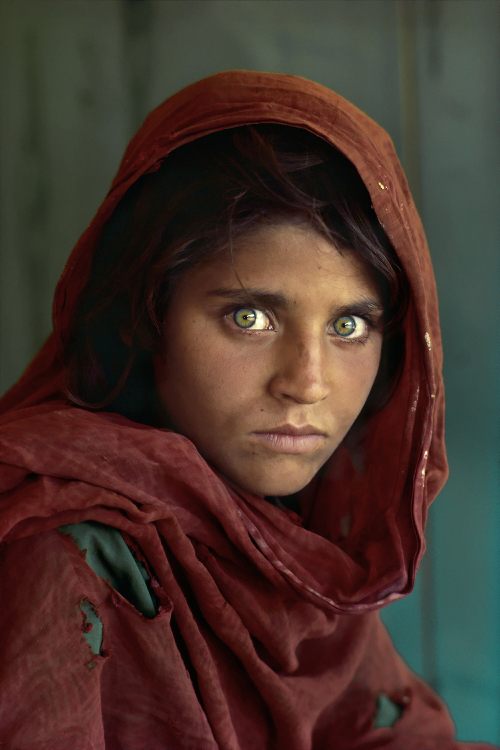
\includegraphics[width=.2 \textwidth]{1.jpg}}
	 {\caption{the Afghani girl}\label{fig:afghanigirl}}
\end{figure}

 Sharbat Gula is an Afghani girl who were living in Afghanistan and moved to Pakistan as a refugee and a famous photo of her were shot on 1984 when she was 12 years old on 2002 the photographer of the photo searched for her in Afghanistan to recapture the effect of time on here and managed to capture another photo of her at the age of about 30.As you can see now on the two images side by side, you cannot believe that  the difference between the two images is only 17 years Figure[ \ref{fig:afghanigirl17years}]
\begin{figure}[hbtp]
	 \centerline{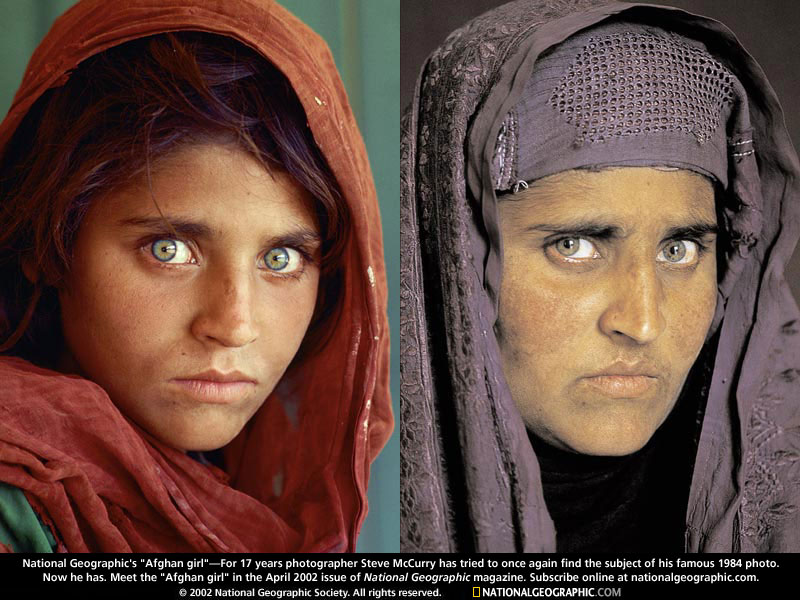
\includegraphics[width=0.4\textwidth]{2.jpg}}
	 {\caption{The Afghani girl between 1984 and 2002.}\label{fig:afghanigirl17years}}
\end{figure}.

Another example is at the most stressful job in the world the president of the united states of America , we will take president Bill Clinton(in office for 8 years 1993-2001) as an example what you are seeing in figure[\ref{fig:clinton}]
\ref{fig:afghanigirl17years}]
\begin{figure}[hbtp]
	 \centerline{\includegraphics[width=0.2\textwidth]{3.jpg}}
	 {\caption{Bill Clinton 1993.}\label{fig:clinton}}
\end{figure}.
 is an official photo at the very early days of his first presidency term and the other photo in figure[\ref{fig:clinton8}]
 \begin{figure}[hbtp]
	 \centerline{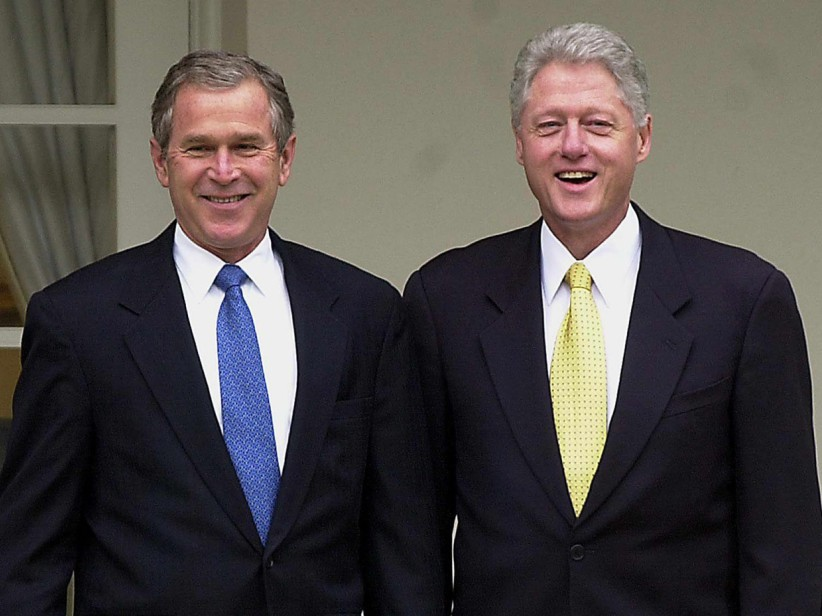
\includegraphics[width=0.3\textwidth]{4.jpg}}
	 {\caption{Bill Clinton 2001.}\label{fig:clinton8}}
\end{figure}.
  is 8 years later while leaving the chair to president George W. Bush. although only 8 years passed between the two photos but the ageing apparent on the face of Clinton maybe interpreted as about 12-16 years. Although it worth mentioning that a "even assuming accelerated ageing during office, most of the presidents who died of natural causes still outlived men who were the same age at their inauguration." \cite{olshansky2011aging}, which is not the case for Sharbat Gula that at the age of 30 with no access to medical care can barely be as outfit as women in her late fifties in other countries.

To this we can conclude that although it's not the only factor but the surrounding stress and living condition can be a great factor of showing the ageing symptoms on a person's outfit even if it's not affecting it's overall health condition with access to medical care.

\end{itemize}


\subsection{Experiment}
\label{sec:model:subsec:experiment}

Nikki Owen has devised a simple experiment using apples in order to prove her hypothesis. she claimed that apples have similar water content -60 percent- to the human body which is false. According to our scientific research, Apples have a water percentage in the range of 81 percent to 84 percent \cite{institute2005dietary}.The total amount of water in a man of average weight is 57 percent of the body weight. while it's 75 percent in a newborn infant \cite{andrew2003diastolic}.

We have applied Owen's experiment with the following procedures: 1) we brought a good condition non-decayed apple 2)wash the apple 3)cut it to two halves (hate, love) using a clean knife 4)we left the apple in the same place for 6 days with the same Environmental conditions and temperature (14 Celsius degree)  [\ref{fig:apple1} ,\ref{fig:apple2}, \ref{fig:apple3}] .

\begin{figure}[hbtp]
	 \centerline{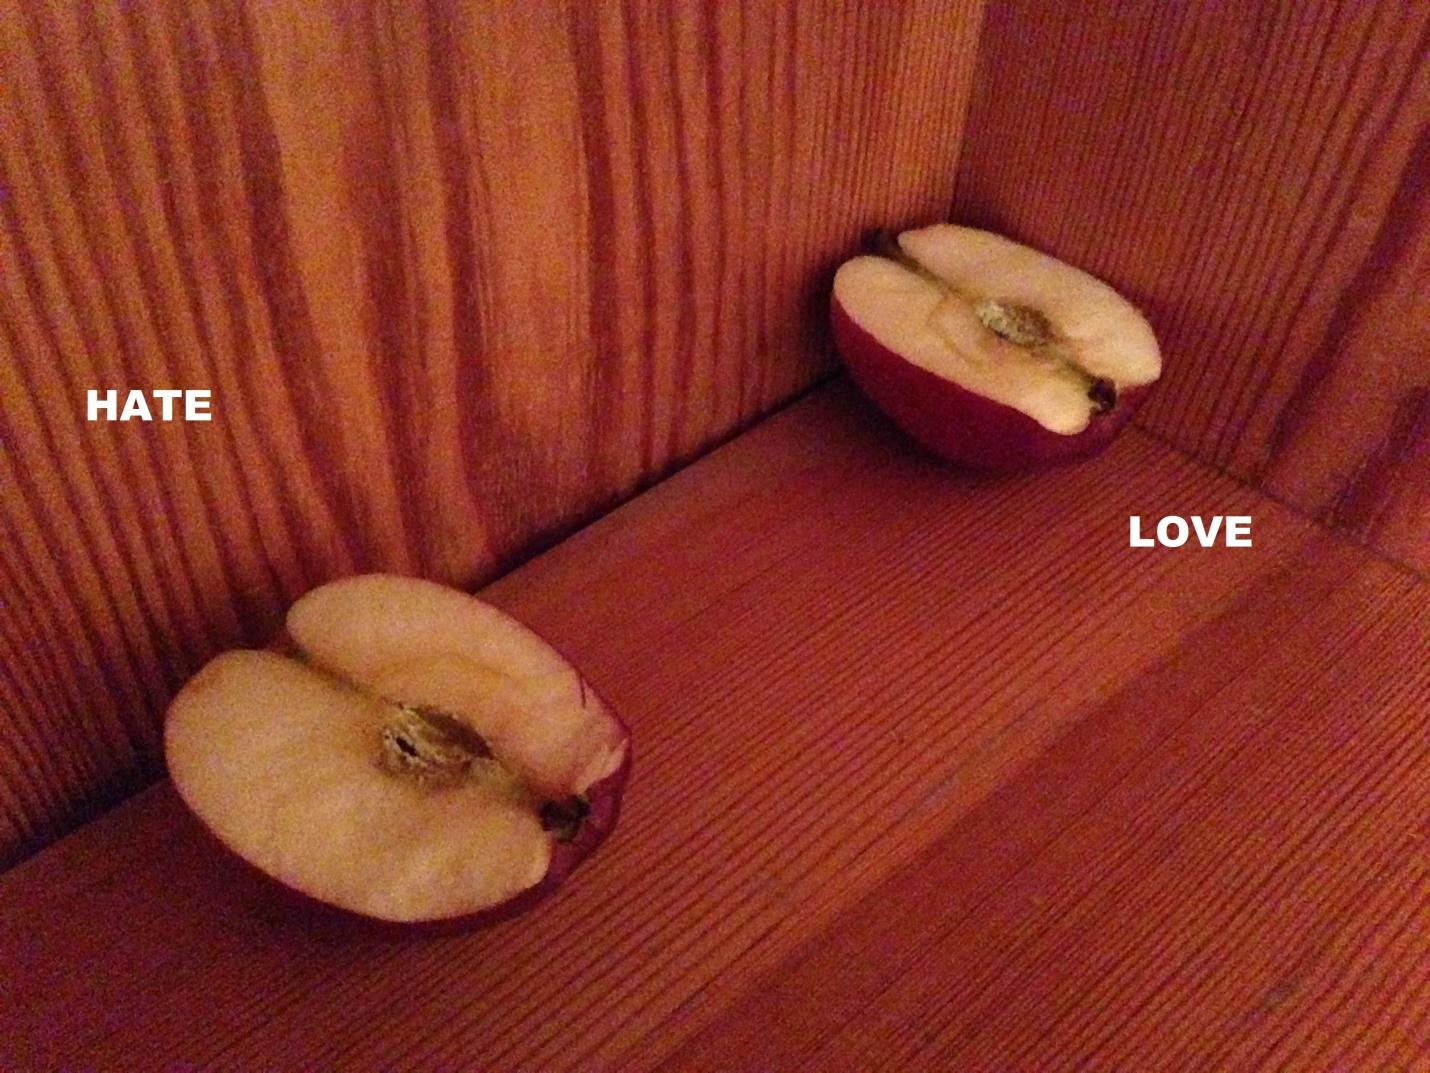
\includegraphics[width=0.3\textwidth]{apple1.jpg}}
	 {\caption{Day (1):The apple after cutting it into two halves.}\label{fig:apple1}}
\end{figure}

\begin{figure}[hbtp]
	 \centerline{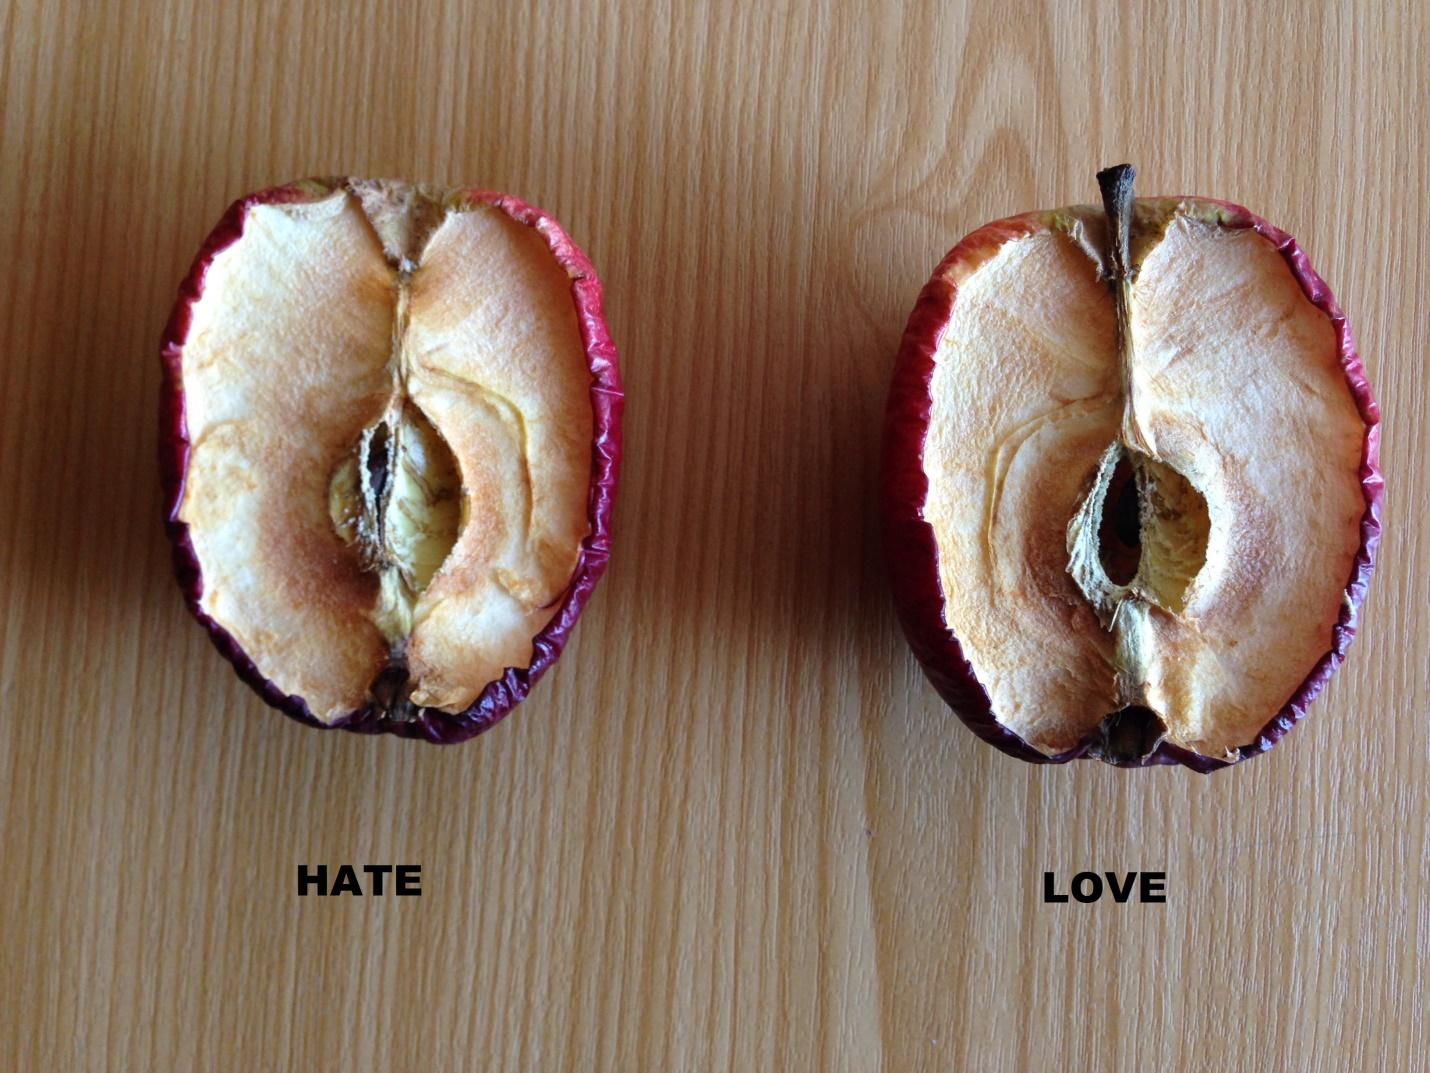
\includegraphics[width=0.3\textwidth]{apple2.jpg}}
	 {\caption{Day (3):The Apple begins to change its color. 17 Celsius degree}\label{fig:apple2}}
\end{figure}

\begin{figure}[hbtp]
	 \centerline{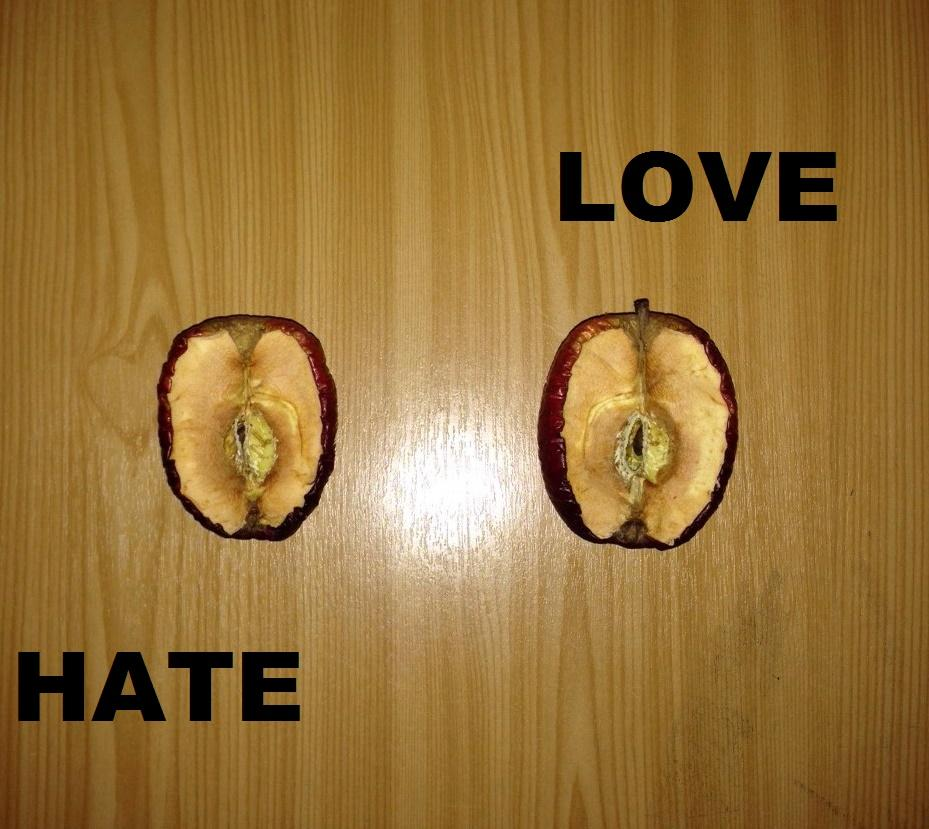
\includegraphics[width=0.3\textwidth]{apple3.jpg}}
	 {\caption{Day (6):The Love half of the apple is darker than the hate one.}\label{fig:apple3}}
\end{figure}

In figure \ref{fig:apple3}, we can see that the apple has one half more decayed than the other. Therefore, we conclude that there are some natural factors affected the apple unequally regardless speaking to it. which clearly shows that Nikki's apple experiment failed to prove her hypothesis. 


\section{Conclusion}
\label{sec:concl}

Through out our scientific research we supported Nikki Owen's hypothesis which stated that "A more youthful appearance could be down to saying kinder things to ourselves and adopting a happier outlook on life" Although we proved that the apple experiment failed to prove her hypothesis.In addition, We included some scientific publications to show the power of positive thinking and the relation between surrounding stresses and ageing symptoms. Although we refused Dr Patrick Bowler's claim about the relation between the positive attitude and the cancerous people. Furthermore, we applied Nikki's experiment regardless speaking to the apple and we concluded that there are some natural factors affected them even if we put them at the same place and environmental conditions.  


%%%%%%%%%%%%%%%%%%%%%%%%%%%%%%%%%%%%%%
% hier werden - zum Ende des Textes - die bibliographischen Referenzen
% eingebunden
%
% Insbesondere stehen die eigentlichen Informationen in der Datei
% ``bib.bib''
%
\bibliography{bib}
\bibliographystyle{plain}

\end{document}


